% Chapter 4 RKNN-TSVM

\chapter{ماشین بردار پشتیبان دو قلو مبتنی بر رگولارسیون و نزدیک‌ترین همسایه}\label{ch:4}
\section{مقدمه}\label{sec:4:1}
در بخش ‏\ref{sec:2:2:3} برخی از گسترش‌های \lr{TSVM} معرفی شد. بعضی از این گسترش‌ها مبتنی بر رویکرد نزدیک‌ترین همسایه هستند. با وجود اینکه گسترش‌های با رویکرد نزدیک‌ترین همسایه مزیت‌هایی مانند دقت بیشتر را دارند، این روش‌ها سه نقطه ضعف دارند که عبارتند از:
\begin{enumerate}
	\item این روش‌ها به نمونه‌ها بر اساس شمارش تعداد همسایه‌های نزدیک‌شان وزن می‌دهند. بطوریکه فاصله بین نزدیک‌ترین همسایه‌های یک نمونه در نظر گرفته نمی‌شود. نسبت دادن وزن براساس فاصله می‌تواند باعث شناسایی بهتر نواحی پرتراکم شود. به عبارت دیگر، وزن بیشتری به یک نمونه با همسایه‌های نزدیک‌تر داده می‌شود تا به یک نمونه با همسایه‌های دورتر.
	\item این روش‌ها همانند \lr{TSVM} خطای آموزشی (ریسک تجربی) را کمینه می‌کنند. از این رو امکان برازش بیش از حد وجود دارد و تعمیم‌پذیری مدل خروجی کاهش می‌یابد. این نقطه ضعف با در نظر گرفتن ریسک ساختاری در تابع هدف مسئله بهینه‌سازی برطرف می‌شود.
	\item در این روش‌ها، گراف نزدیک‌ترین همسایه با الگوریتم جستجوی کامل\footnote{\lr{Full search algorithm}}  (\lr{FSA}) ساخته می‌شود. مرتبه زمانی این الگوریتم جستجو برابر با  $\mathcal{O}(m^2)$ است. بنابراین اجرای این الگوریتم روی مجموعه داده‌های بزرگ زمان‌بر خواهد بود. اگرچه الگوریتم‌های جدیدی برای ساخت گراف نزدیک‌ترین همسایه ارائه شده است که مرتبه زمانی کمتر از روش \lr{FSA} دارند. در سال 2015، الگوریتم گراف نزدیک‌ترین همسایه مبتنی بر تفاوت مکانی فاصله‌ها\footnote{\lr{Location difference of multiple distances based k-nearest neighbors algorithm (LDMDBA)}}  (\lr{LDMDBA}) ارائه شد \cite{xia2015}. مرتبه زمانی روش \lr{LDMDBA} برابر با $\mathcal{O}(\log nm\log m)$ است. این روش جدید می‌تواند به منظور ساخت گراف نزدیک‌ترین همسایه استفاده شود. در نتیجه پیچیدگی محاسباتی کلی دسته بند بهبود می‌یابد.
\end{enumerate} 

در این فصل، با انگیزه‌ی برطرف کردن نقاط ضعف اشاره شده، دسته‌بند ماشین بردار پشتیبان دو قلو مبتنی بر رگولارسیون و نزدیک‌ترین همسایه  (\lr{RKNN-TSVM}) ارائه شده است. روش پیشنهادی برخلاف روش‌های \lr{WLTSVM} و \lr{KNN-LSTSVM}، به نمونه‌های آموزشی بر اساس فاصله بین نزدیک‌ترین همسایه‌هایش وزن می‌دهد. بطوریکه شناسایی نمونه‌های با تراکم بالا و فشردگی درون کلاسی بهبود می‌یابد. همچنین روش \lr{RKNN-TSVM} ریسک ساختاری را کمینه می‌کند. بنابراین مسائل بهینه‌سازی در این روش معین مثبت  \footnote{\lr{Positive definite}}هستند.

چالش اصلی روش \lr{RKNN-TSVM}، پیچیدگی محاساباتی بالا برای مجموعه داده‌های بزرگ است. زیرا این روش دو مسئله بهینه‌سازی دوگان حل می‌کند و همچنین \lr{k} نزدیک‌ترین همسایه برای تمام نمونه‌های آموزشی باید محاسبه شود. به منظور بهبود مرتبه زمانی گراف نزدیک‌ترین همسایه، روش‌هایی مانند درخت \lr{k} بعدی\footnote{\lr{K-dimensional tree}}  (\lr{k-d tree}) \cite{friedman1977}، درخت \lr{LB}\footnote{\lr{Lower bound tree}}  \cite{chen2007} و روش \lr{LDMDBA} ارائه شده است. روش \lr{LDMDBA} دارای مرتبه زمانی  $\mathcal{O}(\log nm\log m)$ است که از روش \lr{FSA} و بیشتر الگوریتم‌های گراف نزدیک‌ترین همسایه بهتر است. روش \lr{RKNN-TSVM} برای ساخت گراف نزدیک‌ترین همسایه از روش \lr{LDMDBA} استفاده می‌کند.

روش ارائه شده در این فصل، یعنی \lr{RKNN-TSVM} دارای مزایای زیر است:  
\begin{itemize}[label=$\bullet$]
	\item	روش \lr{RKNN-TSVM} به نمونه‌ها براساس فاصله نزدیک‌ترین همسایه‌هایش وزن می‌دهد. به عبارت دیگر، نواحی پرتراکم بهتر شناسایی می‌گردد و ابرصفحه به نمونه‌های با تراکم بالا نزدیک‌تر می‌شود. بطوریکه به نمونه‌های با همسایه‌های نزدیک‌تر وزن بیشتری نسبت داده می‌شود.
	\item برخلاف روش \lr{WLTSVM} و \lr{KNN-LSTSVM}، ریسک ساختاری در مسائل بهینه‌سازی روش \lr{RKNN-TSVM} لحاظ شده است. بدین ترتیب دقت و تعمیم‌پذیری مدل خروجی افزایش بهبود می‌یابد.
	\item روش \lr{LDMDBA} جهت بهبود پیچیدگی محاسباتی دسته‌بند بکار گرفته شده است. همچنین این روش برای نسخه غیر خطی دسته‌بند \lr{RKNN-TSVM} نیز موثر می‌باشد. بطوریکه پیدا کردن \lr{k} نزدیک‌ترین همسایه در فضای ویژگی با ابعاد بسیار بالا توسط روش \lr{LDMDBA} بسیار سریعتر از روش \lr{FSA} است.
	\item شیوه وزن‌دهی به یک نمونه در روش \lr{RKNN-TSVM}، براساس فاصله نمونه مورد نظر از نزدیک‌ترین همسایه‌هایش است. بطوریکه مدل خروجی حساسیت کمتری نسبت به نمونه‌های نویزی و پرت دارد.
\end{itemize}

در ادامه این فصل، ابتدا روش \lr{LDMDBA} به طور خلاصه معرفی می‌شود. شیوه جدید وزن دهی در بخش بیان شده است. نسخه خطی و غیر خطی روش \lr{RKNN-TSVM} شرح داده می‌شود. سپس روش \lr{RKNN-TSVM} در بخش تحلیل و بررسی می‌شود.

\section{الگوریتم نزدیک‌ترین همسایه مبتنی بر تفاوت مکانی فاصله‌ها}\label{sec:4:2}
الگوریتم \lr{LDMDBA} مفهوم تفاوت مکانی را معرفی کرد \cite{xia2015}. ایده اصلی این است که همسایه‌ها راجع به مکان‌شان اطلاعات مشابه‌ای دارند. به منظور شرح بهتر، شکل \ref{fig:LDMDBA}  ایده روش \lr{LDMDBA} را نشان می‌دهد.

\begin{figure}[!b]
	\centering
	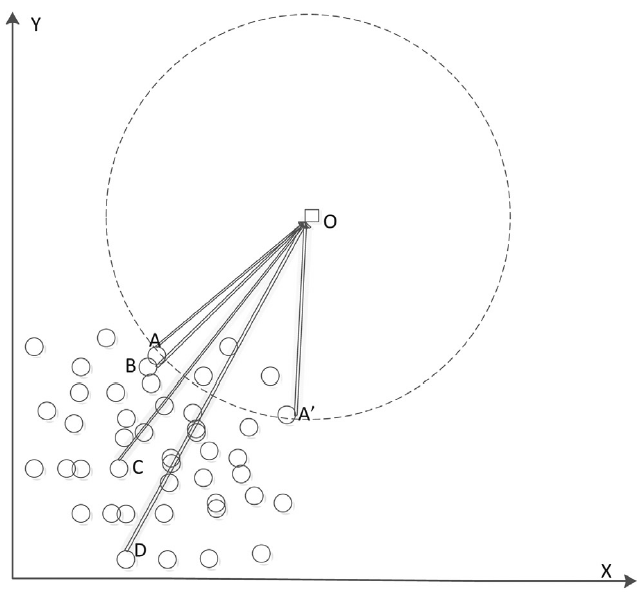
\includegraphics[scale=0.5]{LDMDBA-Idea}
	\caption{ایده اصلی روش \lr{LDMDBA} \cite{xia2015}}
	\label{fig:LDMDBA}
\end{figure}

همانطور که در شکل  \ref{fig:LDMDBA}‏ نشان داده شده است، تفاوت مکانی همسایه‌ها از طریق فاصله آن‌ها از نقطه مرجع $O$ اندازه‌گیری می‌شود. برای مثال، نمونه  $A$ همسایه نزدیک نمونه $B$  است. زیرا فاصله هر دو نمونه از نقطه مرجع  بسیار مشابه یکدیگر است. با این حال فاصله از یک نقطه مرجع برای پیدا کردن دقیق نزدیک‌ترین همسایه‌ها کافی نمی‌باشد. بنابراین فاصله از چندین نقطه مرجع محاسبه می‌شود.

به منظور بیان الگوریتم \lr{LDMDBA}، مسئله پیدا کردن  $k$نزدیک‌ترین همسایه با مجموعه داده $T=\{(x_1, y_1),\dots,(x_m, y_m)\}$ را در نظر می‌گیریم. فاصله یک نمونه   $x_{j} \in T$ از نقطه مرجع $O_{1}$  به این صورت $Dis_{1}(x_{j})=\left\|x_{j}-O_{1}\right\|$  نشان داده می‌شود. . تعداد نقاط مرجع طبق مقاله اصلی \cite{xia2015} برابر با  ${{\log }_{2}}n$ است ($n$  بیانگر تعداد ویژگی‌ها است.). مقادیر $i$ بعد اول  $i$مین نقطه مرجع $O_{i}$  مساوی با 1- و سایر مقادیر برابر با 1 است. به عبارت دیگر، نقطه مرجع  $i$ام به این صورت   $O_{i}=(-1,-1,\dots,-1,1,\dots,1)$ است. همچنین $Nea_{i}(x_{j})$ نشان‌دهنده همسایه‌های نمونه $x_j$ است که توسط نقطه مرجع $i$ام مشخص شده است.

به منظور بدست آوردن مجموعه  $Nea_{i}(x_{j})$ ، ابتدا فاصله نمونه  $x_j$ از تمام نقاط مرجع محاسبه می‌شود. بعد از مرتب‌سازی فاصله‌ها، یک دنبال مرتب شده بدست می‌آید. بطوریکه $k$نزدیک‌ترین همسایه نمونه $x_j$  در یک زیردنباله با مرکزیت نمونه  $x_j$  قرار دارد. طول زیردنباله برابر با  $2k*\varepsilon$ است. بطوریکه مقدار $\varepsilon$  مساوی با  ${{\log }_{2}}{{\log }_{2}}m$ می‌باشد (نحوه انتخاب مقدار $\varepsilon$  در مقاله اصلی \cite{xia2015} ذکر شده است.).  در آخر، فاصله اقلیدسی تمام نمونه‌ها در زیردنباله محاسبه می‌شود. آن دسته از نمونه‌های متناظر با  $k$کوچک‌ترین فاصله در زیردنباله به عنوان $k$نزدیک‌ترین همسایه نمونه $x_j$ شناخته می‌شوند. در جمع‌بندی این بخش، الگوریتم \lr{LDMDBA} به صورت گام به گام بیان می‌شود.

\begin{algo}
	الگوریتم نزدیک‌ترین همسایه مبتنی بر تفاوت مکانی فاصله‌ها (\lr{LDMDBA})
	
	ابتدا مجموعه آموزشی $T$ را در نظر می‌گیریم. سپس مقدار $k$ یعنی تعداد نزدیک‌ترین همسایه‌ها مشخص می‌گردد. با در نظرگرفتن $i=1$،  $k$نزدیک‌ترین همسایه با طی کردن گام‌های زیر بدست می‌آید.
	
	\begin{enumerate}
		\item  $i$مین نقطه مرجع  $O_{i}$ به عنوان یک بردار در نظر گرفته می‌شود که   $i$بعد اول آن برابر 1- است. سایر مقادیر این بردار را مقادیر 1 تشکیل می‌دهد.
		\item 	فاصله تمام نمونه‌ها از نقطه مرجع $O_{i}$  با استفاده از $Dis_{i}(x_{j})=\left\|x_{j}-O_{i}\right\|$  محاسبه می‌شود.
		\item 	تمام نمونه‌ها بر اساس مقدار $Dis_{i}$  مرتب می‌شود و یک دنباله مرتب شده بدست می‌آید.
		\item 	یک زیردنباله‌ای از نمونه‌ها با اندازه  $2k*{{\log }_{2}}{{\log }_{2}}m$ و  $x_{j}$ به عنوان نمونه مرکز را در نظر گرفته می‌شود. سپس فاصله اقلیدسی نمونه  $x_{j}$ از تمام نمونه‌های زیردنباله محاسبه می‌گردد.
		\item فاصله‌های محاسبه شده در گام 4 مرتب می‌شود.
		\item  $k$کوچک‌ترین فاصله در زیردنباله مرتب شده،  $k$نزدیک‌ترین همسایه نمونه  $x_{j}$ هستند.
		\item چنانچه همسایه تمام نمونه‌ها با استفاده از همه نقاط مرجع محاسبه گردد، الگوریتم خاتمه می‌یابد. در غیر این صورت،  $i=i+1$ و الگوریتم در گام 1 ادامه می‌یابد.
	\end{enumerate}
\end{algo}

مرتبه زمانی الگوریتم \lr{LDMDBA} توسط گام‌های 3 و 5 مشخص می‌شود. مرتبه زمانی الگوریتم مرتب‌سازی استفاده شده در این گام‌ها برابر با   $\mathcal{O}(m{{\log }_{2}}m)$ است. بنابراین پیچیدگی محاسباتی کلی الگوریتم \lr{LDMDBA} مساوی با  $\mathcal{O}(\log nm\log m)$ خواهد بود. مرتبه زمانی الگوریتم \lr{FSA} برابر با  $\mathcal{O}({{m}^{2}}{{\log }_{2}}m)$ است که از الگوریتم \lr{LDMDBA } بیشتر است.

مزیت مهم دیگر الگوریتم \lr{LDMDBA} این است که از ساختار درختی استفاده نمی‌کند. درنتیجه این الگوریتم برای داده‌های با ابعاد بسیار بالا موثر است. نتایج ارزیابی در مقاله اصلی \cite{xia2015}، برتری این الگوریتم را نسبت به \lr{FSA} و سایر الگوریتم‌های نزدیک‌ترین همسایه نشان می‌دهد.